\documentclass[aspectratio=169,12pt]{beamer}
\usetheme{Madrid}
\usecolortheme{dolphin}
\usefonttheme{professionalfonts}
\setbeamertemplate{navigation symbols}{}
\setbeamertemplate{footline}{}

\usepackage[T1]{fontenc}
\usepackage[utf8]{inputenc}
\usepackage{graphicx}
\usepackage{amsmath,amssymb}
\usepackage{hyperref}
\usepackage{physics}
\usepackage{tikz}
\usetikzlibrary{angles,quotes}

\title{Introduction to Complex Numbers}
\author{JAMOTTE Maxime, SCHOONEN Cédric}
\institute{Digital Learning Hub}
\date{}

\begin{document}

\begin{frame}
  \titlepage
\end{frame}

\begin{frame}{Table of Contents}
  \tableofcontents
\end{frame}

\section{Motivation}

\begin{frame}{Exponentiation of real numbers}

  Squaring:

  \begin{center}
  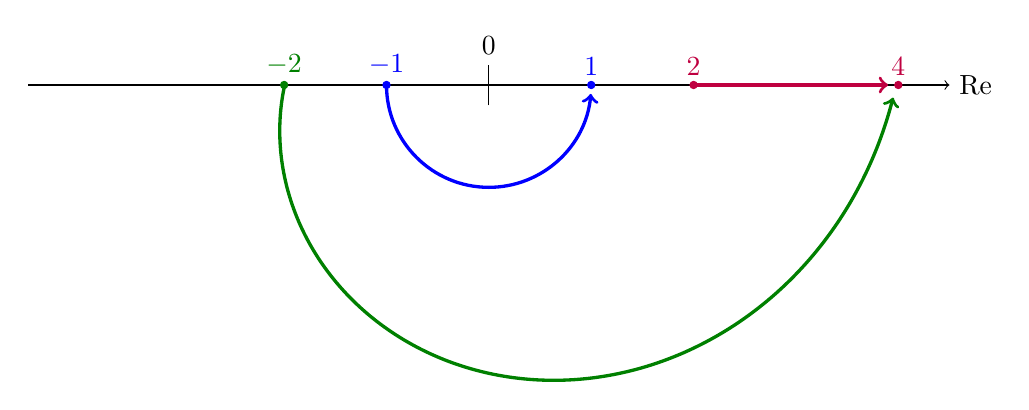
\begin{tikzpicture}[scale=1.3]
    \draw[->] (-4.5,0) -- (4.5,0) node[right] {Re};
    \draw[-] (0,-0.2) -- (0,0.2) node[above] {$0$};
    \draw[->,very thick,purple] (2,0) -- (3.9,0);
    \draw[->,very thick,blue] (-1,0) arc (180:355:1.0);
    \draw[->,very thick,green!50!black,domain=pi:2*pi-0.03,samples=100,smooth,variable=\t] 
  plot ({exp(\t/4.55)*cos(\t r)}, {exp(\t/4.55)*sin(\t r)});
    \filldraw[blue] (-1,0) circle (1pt) node[above] {$-1$};
    \filldraw[blue] (1,0) circle (1pt) node[above] {$1$};
    \filldraw[purple] (2,0) circle (1pt) node[above] {$2$};
    \filldraw[purple] (4,0) circle (1pt) node[above] {$4$};
    \filldraw[green!50!black] (-2,0) circle (1pt) node[above] {$-2$};
  \end{tikzpicture}
  \end{center}

\end{frame}

\begin{frame}{Exponentiation des nombres réels}

  \begin{center}
  \begin{tikzpicture}[scale=1.9]
    \draw[->] (-2.5,0) -- (2.5,0) node[right] {Re};
    \draw[-] (0,-0.2) -- (0,0.2) node[above] {$0$};
    \draw[->,very thick,purple] (1,0) arc (0:172:1.0) node[midway,above] {$(-1)^{1, 3, 5, \dots}$};
    \draw[->,very thick,blue] (-1,0) arc (180:352:1.0) node[midway,below] {$(-1)^{2, 4, 6, \dots}$};
    \filldraw[black] (-1,0) circle (1pt) node[above left] {$-1$};
    \filldraw[black] (1,0) circle (1pt) node[above right] {$1$};
  \end{tikzpicture}
  \end{center}

\end{frame}

\begin{frame}{No fractional exponent for negative numbers?}

  \begin{center}
  \begin{tikzpicture}[scale=1.9]
    \draw[->] (-2.5,0) -- (2.5,0) node[right] {Re};
    \draw[-] (0,-0.2) -- (0,0.2) node[above] {$0$};
    \draw[->,very thick,purple] (1,0) arc (0:82:1.0) node[midway, above right] {$(-1)^{1/2}$ ?};
    \draw[->,very thick,blue] (-1,0) arc (180:352:1.0) node[midway,below] {$(-1)^2$};
    \filldraw[black] (-1,0) circle (1pt) node[above left] {$-1$};
    \filldraw[black] (1,0) circle (1pt) node[above right] {$1$};
    \filldraw[purple] (0,1) circle (1pt);
  \end{tikzpicture}
  \end{center}

\end{frame}

\begin{frame}{We complete with an imaginary axis}

  \begin{center}
  \begin{tikzpicture}[scale=1.9]
    \draw[->] (-2.5,0) -- (2.5,0) node[right] {Re};
    \draw[->] (0,-1.5) -- (0,1.5) node[above] {Im};
    \draw[->,very thick,purple] (1,0) arc (0:82:1.0) node[midway, above right] {$(-1)^{1/2}$};
    \filldraw[black] (-1,0) circle (1pt) node[above left] {$-1$};
    \filldraw[black] (1,0) circle (1pt) node[above right] {$1$};
    \filldraw[purple] (0,1) circle (1pt) node[above left] {$i$};
    \filldraw[purple] (0,-1) circle (1pt) node[below left] {$-i$};
  \end{tikzpicture}
  \end{center}

\end{frame}

\begin{frame}{We complete with an imaginary axis}

  \begin{center}
  \begin{tikzpicture}[scale=1.9]
    \draw[->] (-2.5,0) -- (2.5,0) node[right] {Re};
    \draw[->] (0,-1.5) -- (0,1.5) node[above] {Im};
    \draw[->,very thick,purple] (1,0) arc (0:262:1.0) node[right] {$\quad (-1)^{3/2}$};
    \filldraw[black] (-1,0) circle (1pt) node[above left] {$-1$};
    \filldraw[black] (1,0) circle (1pt) node[above right] {$1$};
    \filldraw[purple] (0,1) circle (1pt) node[above left] {$i$};
    \filldraw[purple] (0,-1) circle (1pt) node[below left] {$-i$};
  \end{tikzpicture}
  \end{center}

\end{frame}

\begin{frame}{We complete with an imaginary axis}

  \begin{center}
  \begin{tikzpicture}[scale=1.9]
    \draw[->] (-2.5,0) -- (2.5,0) node[right] {Re};
    \draw[->] (0,-1.5) -- (0,1.5) node[above] {Im};
    \draw[gray] (0,0) circle (1);
    \draw[-,very thick,blue] (0,0) -- ({cos(60)},{sin(60)});
    \draw[-,very thick,blue] (0.3,0) arc (0:60:0.3) node[midway, above right] {$\theta$};
    \filldraw[black] (-1,0) circle (1pt) node[above left] {$-1$};
    \filldraw[black] (1,0) circle (1pt) node[above right] {$1$};
    \filldraw[black] (0,1) circle (1pt) node[above left] {$i$};
    \filldraw[black] (0,-1) circle (1pt) node[below left] {$-i$};
    \filldraw[blue] ({cos(60)},{sin(60)}) circle (1pt) node[above right] {$(-1)^{\theta/\pi}$};
  \end{tikzpicture}
  \end{center}

\end{frame}

\begin{frame}{Each real number is "augmented" with a phase}

  \begin{center}
  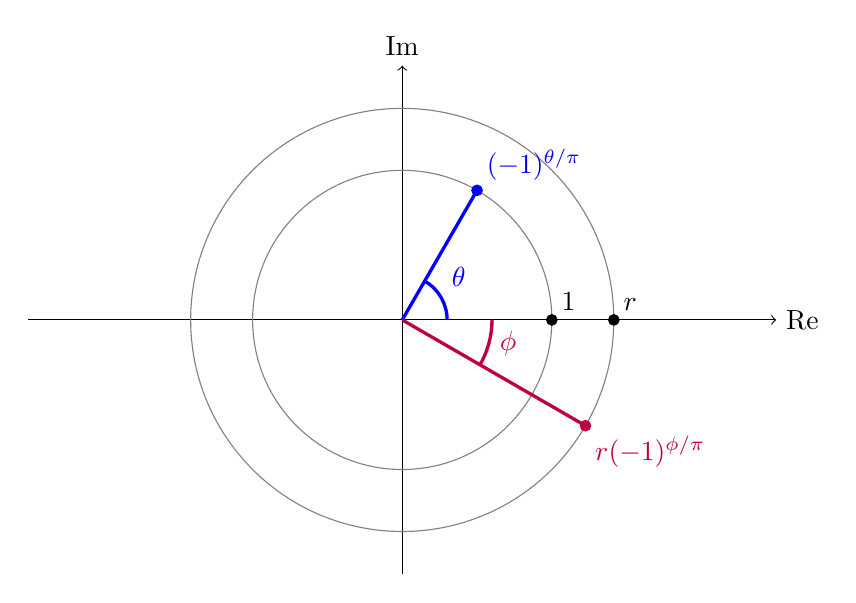
\begin{tikzpicture}[scale=1.9]
    \draw[->] (-2.5,0) -- (2.5,0) node[right] {Re};
    \draw[->] (0,-1.7) -- (0,1.7) node[above] {Im};
    \draw[gray] (0,0) circle (1);
    \draw[gray] (0,0) circle (1.4142);
    \draw[-,very thick,blue] (0,0) -- ({cos(60)},{sin(60)});
    \draw[-,very thick,purple] (0,0) -- ({1.4142*cos(-30)},{1.4142*sin(-30)});
    \draw[-,very thick,blue] (0.3,0) arc (0:60:0.3) node[midway, above right] {$\theta$};
    \draw[-,very thick,purple] (0.6,0) arc (0:-30:0.6) node[midway, right] {$\phi$};
    %\filldraw[black] (-1,0) circle (1pt) node[above left] {$-1$};
    \filldraw[black] (1,0) circle (1pt) node[above right] {$1$};
    \filldraw[black] (1.4142,0) circle (1pt) node[above right] {$r$};
    %\filldraw[black] (0,1) circle (1pt) node[above left] {$i$};
    %\filldraw[black] (0,-1) circle (1pt) node[below left] {$-i$};
    \filldraw[blue] ({cos(60)},{sin(60)}) circle (1pt) node[above right] {$(-1)^{\theta/\pi}$};
    \filldraw[purple] ({1.4142*cos(-30)},{1.4142*sin(-30)}) circle (1pt) node[below right] {$r(-1)^{\phi/\pi}$};
  \end{tikzpicture}
  \end{center}

\end{frame}

\begin{frame}{Each real number is "augmented" with a phase}

  \begin{center}
  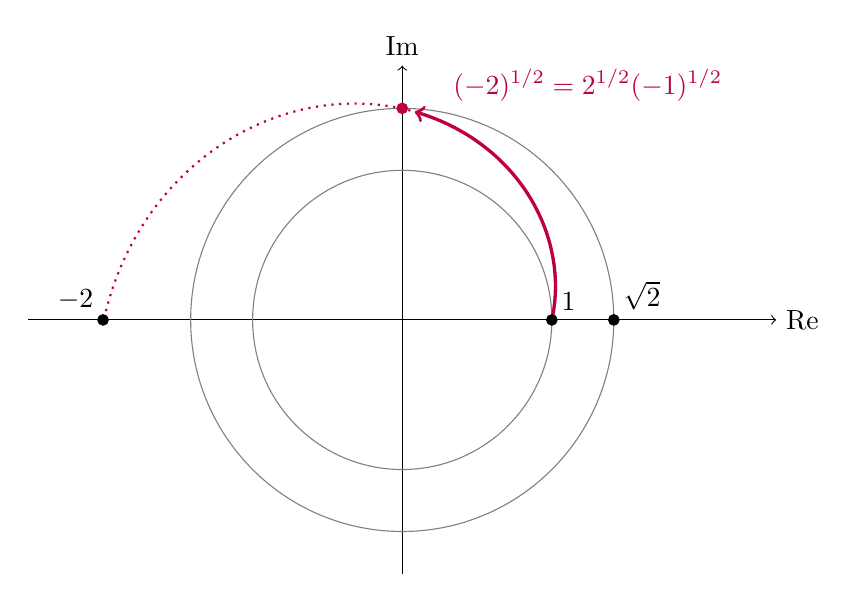
\begin{tikzpicture}[scale=1.9]
    \draw[->] (-2.5,0) -- (2.5,0) node[right] {Re};
    \draw[->] (0,-1.7) -- (0,1.7) node[above] {Im};
    \draw[gray] (0,0) circle (1);
    \draw[gray] (0,0) circle (1.4142);
    \draw[dotted,thick,purple,domain=0:pi,samples=100,smooth,variable=\t] 
  plot ({exp(\t/4.55)*cos(\t r)}, {exp(\t/4.55)*sin(\t r)});
    \draw[->,very thick,purple,domain=0:pi/2-0.06,samples=100,smooth,variable=\t] 
  plot ({exp(\t/4.55)*cos(\t r)}, {exp(\t/4.55)*sin(\t r)}) node[above right] {$\quad (-2)^{1/2} = 2^{1/2}(-1)^{1/2}$};
    \filldraw[black] (-2,0) circle (1pt) node[above left] {$-2$};
    \filldraw[black] (1,0) circle (1pt) node[above right] {$1$};
    \filldraw[black] (1.4142,0) circle (1pt) node[above right] {$\sqrt{2}$};
    \filldraw[purple] (0,1.4142) circle (1pt);
  \end{tikzpicture}
  \end{center}

\end{frame}

\begin{frame}{Multiplication of complex numbers}

  \begin{center}
  \begin{itemize}
    \item A complex number combines a \textbf{magnitude} (length) and a \textbf{phase} (angle):
    \begin{equation*}
      z = r (-1)^{\theta/\pi}
    \end{equation*}
    \item Multiplication of two complex numbers:
    \begin{equation*}
      z_1 z_2 = r_1 (-1)^{\theta_1/\pi} r_2 (-1)^{\theta_2/\pi} = r_1 r_2 (-1)^{(\theta_1+\theta_2)/\pi}
    \end{equation*}
    \item Division of two complex numbers:
    \begin{equation*}
      \frac{z_1}{z_2} = \frac{r_1 (-1)^{\theta_1/\pi}}{r_2 (-1)^{\theta_2/\pi}} = \frac{r_1}{r_2} (-1)^{(\theta_1-\theta_2)/\pi}
    \end{equation*}
  \end{itemize}
  \end{center}

\end{frame}

\begin{frame}{Exponentiation of complex numbers}

  \begin{center}
  \begin{itemize}
    \item Exponentiation by a real number:
    \begin{equation*}
      z^a = \left( r (-1)^{\theta/\pi} \right)^a = r^a (-1)^{a\theta/\pi}
    \end{equation*}
    \item n-th roots:
    \begin{equation*}
      \sqrt[n]{z} = \left( r (-1)^{\theta/\pi} \right) ^{1/n} = \sqrt[n]{r} (-1)^{\theta/n\pi}
    \end{equation*}
    \bigskip
    \item What about exponentiation by a complex number?
    \begin{equation*}
      z^i = ??
    \end{equation*}
  \end{itemize}
  \end{center}

\end{frame}

\begin{frame}{Complex exponents}

  \begin{center}
  \begin{itemize}
    \item Euler's formula: \hspace{5mm} $\boxed{e^{i\pi} = -1}$ 
    \begin{flushright}
      ... a bit long to explain
    \end{flushright}
    \bigskip
    \item Allows rewriting our phases $(-1)^{\theta/\pi}$ as $e^{i\theta}$
    \bigskip
    \item Conventional notation for complex numbers: \hspace{5mm} $\boxed{z = r e^{i\theta}}$
    %\item Donne lieu à la notation polaire: $\boxed{z = r e^{i\theta}}$ car nos phases $(-1)^{\theta/\pi}$ se notent $e^{i\theta}$
    % \begin{flushright}
    %   ... car nos phases $(-1)^{\theta/\pi}$ se notent alors $e^{i\theta}$
    % \end{flushright}
  \end{itemize}
  \end{center}

\end{frame}

\begin{frame}{Multiplication of complex numbers (Euler)}

  \begin{center}
  \begin{itemize}
    \item A complex number combines a \textbf{magnitude} (length) and a \textbf{phase} (angle):
    \begin{equation*}
      z = r e^{i\theta}
    \end{equation*}
    \item Multiplication of two complex numbers:
    \begin{equation*}
      z_1 z_2 = r_1 e^{i\theta_1} r_2 e^{i\theta_2} = r_1 r_2 e^{i(\theta_1+\theta_2)}
    \end{equation*}
    \item Division of two complex numbers:
    \begin{equation*}
      \frac{z_1}{z_2} = \frac{r_1 e^{i\theta_1}}{r_2 e^{i\theta_2}} = \frac{r_1}{r_2} e^{i(\theta_1-\theta_2)}
    \end{equation*}
  \end{itemize}
  \end{center}

\end{frame}

\begin{frame}{Exponentiation of complex numbers (Euler)}

  \begin{center}
  \begin{itemize}
    \item Exponentiation by a real number:
    \begin{equation*}
      z^a = \left( r e^{i\theta} \right)^a = r^a e^{ia\theta}
    \end{equation*}
    \item n-th roots:
    \begin{equation*}
      \sqrt[n]{z} = \left( r e^{i\theta} \right) ^{1/n} = \sqrt[n]{r} e^{i\theta}
    \end{equation*}
    \bigskip
    \item What about exponentiation by a complex number?
    \begin{equation*}
      z^i = e^{\ln(z^i)} = e^{i\ln(z)}
    \end{equation*}
  \end{itemize}
  \end{center}

\end{frame}

\section{Cartesian/vector representation}

\begin{frame}{Three representations}
  
  \bigskip
  \textbf{Cartesian form:}
  \[
    z = x + yi
  \]
  
  \textbf{Vector form:}
  \[
    z = \begin{pmatrix} x \\ y \end{pmatrix}
  \]
  
  \textbf{Polar form:}
  \[
    z = |z| e^{i\theta}
  \]
\end{frame}

\begin{frame}{Cartesian/vector representation}
  
  %$z = x + yi$ avec $x$ la partie réelle et $y$ la partie imaginaire.
  
  \bigskip
  \begin{center}
  \begin{tikzpicture}[scale=1.8]
    \draw[->] (-0.5,0) -- (3.5,0) node[right] {Re};
    \draw[->] (0,-0.5) -- (0,2.5) node[above] {Im};
    \draw[->,thick,blue] (0,0) -- (2.5,1.5);
    \draw[dashed] (2.5,0) node[below] {$x$} -- (2.5,1.5);
    \draw[dashed] (0,1.5) node[left] {$y$} -- (2.5,1.5);
    \filldraw[blue] (2.5,1.5) circle (2pt) node[above right] {$z = x + yi$};
  \end{tikzpicture}
  \end{center}
\end{frame}

\begin{frame}{Addition and subtraction}
  %L'addition se fait composante par composante:
  \[
    (x_1 + y_1 i) + (x_2 + y_2 i) = (x_1+x_2) + (y_1+y_2)i \qquad     \begin{pmatrix} x_1 \\ y_1 \end{pmatrix} + \begin{pmatrix} x_2 \\ y_2 \end{pmatrix} = \begin{pmatrix} x_1 + x_2 \\ y_1 + y_2 \end{pmatrix}
  \]
  
  \begin{center}
  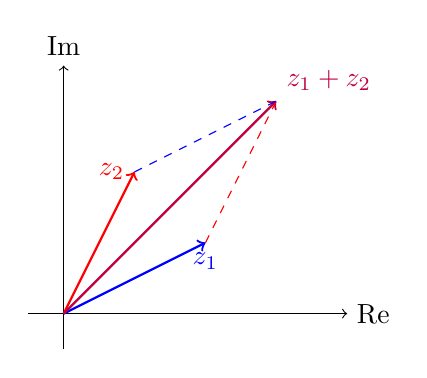
\begin{tikzpicture}[scale=0.9]
    \draw[->] (-0.5,0) -- (4,0) node[right] {Re};
    \draw[->] (0,-0.5) -- (0,3.5) node[above] {Im};
    \draw[->,thick,blue] (0,0) -- (2,1) node[below] {$z_1$};
    \draw[->,thick,red] (0,0) -- (1,2) node[left] {$z_2$};
    \draw[->,thick,purple] (0,0) -- (3,3) node[above right] {$z_1+z_2$};
    \draw[dashed,red] (2,1) -- (3,3);
    \draw[dashed,blue] (1,2) -- (3,3);
  \end{tikzpicture}
  \end{center}
  
\end{frame}

\begin{frame}{Multiplication in Cartesian form}
  Multiplication uses the property $i^2 = -1$:
  \begin{align*}
    (x_1 + y_1 i)(x_2 + y_2 i) 
    %&= x_1 x_2 + x_1 y_2 i + y_1 i x_2 + y_1 y_2 i^2 \\
    &= x_1 x_2 + x_1 y_2 i + y_1 x_2 i + y_1 y_2 (-1) \\
    &= (x_1 x_2 - y_1 y_2) + (x_1 y_2 + y_1 x_2)i
  \end{align*}
  
  \bigskip
  \textbf{Example:}
  \[
    (2 + 3i)(1 + 4i) = (2 \cdot 1 - 3 \cdot 4) + (2 \cdot 4 + 3 \cdot 1)i = -10 + 11i
  \]
\end{frame}

\section{Connection with rotations}

\begin{frame}{Multiplication by $i$}

  \vspace{-5mm}
  \[
    i \cdot (x + yi) = ix + yi^2 = ix - y = -y + xi
  \]
  
  \begin{center}
  \begin{tikzpicture}[scale=1.3]
    \draw[->] (-2.5,0) -- (2.5,0) node[right] {Re};
    \draw[->] (0,-0.5) -- (0,2.5) node[above] {Im};
    \draw[->,thick,blue] (0,0) -- (2,1) node[right] {$z$};
    \draw[->,thick,red] (0,0) -- (-1,2) node[above left] {$iz$};
    \draw[->] (0.8,0.4) arc (25:115:0.9);
    \node at (0.5,1.1) {90°};
  \end{tikzpicture}
  \end{center}
  
  \textbf{90° rotation} counterclockwise.
\end{frame}

\begin{frame}{Multiplication by $1+i$}

  Multiplication by $i$ followed by addition: $(1 + i)z = z + iz$.

  \begin{center}
  \begin{tikzpicture}[scale=1.3]
    \draw[->] (-2.5,0) -- (2.5,0) node[right] {Re};
    \draw[->] (0,-0.5) -- (0,2.5) node[above] {Im};
    \draw[->,thick,blue] (0,0) -- (2,1) node[right] {$z$};
    \draw[->,dashed,red] (0,0) -- (-1,2) node[above left] {$iz$};
    \draw[->,dashed,blue] (-1,2) -- (1,3);
    \draw[->,thick,purple] (0,0) -- (1,3) node[right] {$z+iz$};
    \draw[->] (0.8,0.4) arc (25:70:0.9);
    \node at (0.9,0.9) {45°};
  \end{tikzpicture}
  \end{center}
  
  \textbf{45° rotation} and \textbf{stretching} of the initial vector.
\end{frame}

\begin{frame}{Modulus and phase}
  The \textbf{modulus} (or norm) measures the length of the vector: $\quad |z| = \sqrt{x^2 + y^2}$
  
  \begin{center}
  \begin{tikzpicture}[scale=1.2]
    \draw[->] (-0.5,0) -- (3.5,0) node[right] {Re};
    \draw[->] (0,-0.5) -- (0,2.5) node[above] {Im};
    \draw[->,thick,blue,line width=1.5pt] (0,0) -- (2.5,1.5) node[midway,above left] {$|z|$};
    \draw[dashed] (2.5,0) node[below] {$x$} -- (2.5,1.5);
    \draw[dashed] (0,1.5) node[left] {$y$} -- (2.5,1.5);
    \draw (0.5,0) arc (0:31:0.5);
    \node at (0.8,0.2) {$\theta$};
  \end{tikzpicture}
  \end{center}

  The \textbf{phase} (or argument) is the angle $\theta$ that the vector makes with the real axis.
\end{frame}

\begin{frame}{Trigonometric interpretation}

  \begin{columns}[T]
    \begin{column}{0.49\textwidth}
      \begin{center}
      \begin{tikzpicture}[scale=1.4]
        \draw[->] (-0.5,0) -- (3.5,0) node[right] {Re};
        \draw[->] (0,-0.5) -- (0,2.5) node[above] {Im};
        \draw[->,thick,blue,line width=1.5pt] (0,0) -- (2.5,1.5) node[midway,above left] {$|z|$};
        \draw[dashed] (2.5,0) node[below] {$x$} -- (2.5,1.5);
        \draw[dashed] (0,1.5) node[left] {$y$} -- (2.5,1.5);
        \draw (0.5,0) arc (0:31:0.5);
        \node at (0.8,0.2) {$\theta$};
      \end{tikzpicture}
      \end{center}
    \end{column}
    \begin{column}{0.49\textwidth}

      A complex number encodes a \\
      rotation and an elongation:
      \[
        z = \underbrace{|z|\cos(\theta)}_{x} + i\underbrace{|z|\sin(\theta)}_{y}
      \]

      \textbf{Normalization} to keep only the \\
      rotation:

      \[
        \frac{z}{|z|} = \cos(\theta) + i\sin(\theta)
      \]

    \end{column}
  \end{columns}

\end{frame}

\section{Complex conjugate and division}

\begin{frame}{Division as inverse rotation}
  
  To invert a rotation by angle $\theta$, we perform a rotation by angle $-\theta$.
  
  \bigskip
  This leads us to the concept of \textbf{complex conjugate}, denoted $z^*$ (or $\bar{z}$):
  \[
    z^* = x - iy
  \]
  
  In trigonometric notation:
  \[
    z^* = |z|\cos(-\theta) + i|z|\sin(-\theta) = |z|\cos(\theta) - i|z|\sin(\theta)
  \]
  
\end{frame}

\begin{frame}{The complex conjugate}
  \begin{center}
  \begin{tikzpicture}[scale=1.2]
    \draw[->] (-0.5,0) -- (3.5,0) node[right] {Re};
    \draw[->] (0,-2,0) -- (0,2) node[above] {Im};
    \draw[->,thick,blue] (0,0) -- (2.5,1.5) node[above right] {$z$};
    \draw[->,thick,red] (0,0) -- (2.5,-1.5) node[below right] {$z^*$};
    \draw[dashed] (2.5,1.5) -- (2.5,-1.5);
    \draw (0.7,0) arc (0:31:0.7);
    \draw (0.7,0) arc (0:-31:0.7);
    \node at (1,0.3) {$\theta$};
    \node at (1,-0.3) {$-\theta$};
  \end{tikzpicture}
  \end{center}
  
  \[
    z \cdot z^* = (x + iy)(x - iy) = x^2 + y^2 = |z|^2
  \]
\end{frame}

\begin{frame}{Division of complex numbers}
  To divide by a complex number, we multiply by the conjugate divided by the squared modulus:
  \[
    \frac{1}{z} = \frac{z^*}{zz^*} = \frac{z^*}{|z|^2} = \frac{x - iy}{x^2 + y^2}
  \]
  
  \bigskip
  To divide two complex numbers:
  \[
    \frac{z_1}{z_2} = \frac{z_1 \cdot z_2^*}{|z_2|^2}
  \]
\end{frame}

\begin{frame}{Detailed division in $x + iy$ notation}
  Let us compute $\frac{z_1}{z_2} = \frac{x_1 + iy_1}{x_2 + iy_2}$:
  
  \begin{align*}
    \frac{x_1 + iy_1}{x_2 + iy_2} &= \frac{(x_1 + iy_1)(x_2 - iy_2)}{(x_2 + iy_2)(x_2 - iy_2)} \\
    &= \frac{(x_1 x_2 + y_1 y_2) + i(y_1 x_2 - x_1 y_2)}{x_2^2 + y_2^2} \\
    &= \frac{x_1 x_2 + y_1 y_2}{x_2^2 + y_2^2} + i\frac{y_1 x_2 - x_1 y_2}{x_2^2 + y_2^2}
  \end{align*}
\end{frame}

\section{Polar representation}

\begin{frame}{Polar notation}

  \bigskip
  The notation $z = |z| e^{i\theta}$ elegantly separates:

  \bigskip
  \begin{itemize}
    \setlength{\itemsep}{1em}
    \item The \textbf{modulus} $|z|$: the amplitude, the length
    \item The \textbf{phase} $\theta$: the angle, the direction
  \end{itemize}

  \begin{flushright}
    \vspace{-35mm}
  \begin{tikzpicture}[scale=1.5]
    \draw[->] (-2.5,0) -- (2.5,0) node[right] {Re};
    \draw[->] (0,-0.5) -- (0,2.5) node[above] {Im};
    \draw[->,thick,blue] (0,0) -- (1,2) node[above right] {$z$};
    \draw[->] (0.8,0.0) arc (0:60:0.8);
    \node at (1.0,0.6) {$e^{i\theta}$};
  \end{tikzpicture}
  \end{flushright}

  The exponential transforms multiplications into sums over angles:
  \[
    z_1 \cdot z_2 = |z_1| e^{i\theta_1} \cdot |z_2| e^{i\theta_2} = |z_1||z_2| e^{i(\theta_1 + \theta_2)}
  \]

\end{frame}

\begin{frame}{Euler's formula}
  \textbf{Euler's formula} establishes the link between the exponential and trigonometric functions:
  \[
    e^{i\theta} = \cos(\theta) + i\sin(\theta)
  \]
  
  \bigskip
  Notable special cases:
  \begin{align*}
    e^{i\pi/2} = i \qquad\qquad
    e^{i\pi} = -1 \qquad\qquad
    e^{2i\pi} = 1 \qquad\qquad
  \end{align*}
\end{frame}

\begin{frame}{Operations in polar notation}
  \textbf{Multiplication:}
  \[
    z_1 \cdot z_2 = (|z_1| e^{i\theta_1})(|z_2| e^{i\theta_2}) = |z_1||z_2| \, e^{i(\theta_1+\theta_2)}
  \]
  
  \textbf{Division:}
  \[
    \frac{z_1}{z_2} = \frac{|z_1| e^{i\theta_1}}{|z_2| e^{i\theta_2}} = \frac{|z_1|}{|z_2|} \, e^{i(\theta_1-\theta_2)}
  \]
  
  \textbf{Power:}
  \[
    z^n = (|z| e^{i\theta})^n = |z|^n e^{in\theta}
  \]
  
  \textbf{n-th root:}
  \[
    \sqrt[n]{z} = |z|^{1/n} e^{i\theta/n}
  \]
\end{frame}

\begin{frame}{Roots of unity}

  \bigskip
  The n-th roots of unity are the solutions of $z^n = 1$: $\quad \omega_k = e^{2\pi i k/n} \quad k\in\mathbb{Z}$

  With $n=6$:
 
  \begin{center}
  \begin{tikzpicture}[scale=1.7]
    \draw[->] (-1.5,0) -- (1.5,0) node[right] {Re};
    \draw[->] (0,-1.5) -- (0,1.5) node[above] {Im};
    \draw[gray] (0,0) circle (1);
    \foreach \k in {0,1,2,3,4,5} {
      \filldraw[blue] ({cos(60*\k)},{sin(60*\k)}) circle (1pt);
      %\draw[->,gray] (0,0) -- ({cos(60*\k)},{sin(60*\k)});
    }
    \node[above right] at (1,0) {$1$};
    \node[above right] at ({cos(60*1)},{sin(60*1)}) {$e^{i\pi/3}$};
    \node[above left] at ({cos(60*2)},{sin(60*2)}) {$e^{i2\pi/3}$};
  \end{tikzpicture}
  \end{center}
  \end{frame}

\section{Going further}

\begin{frame}{Videos by 3Blue1Brown} 
  \begin{center}
    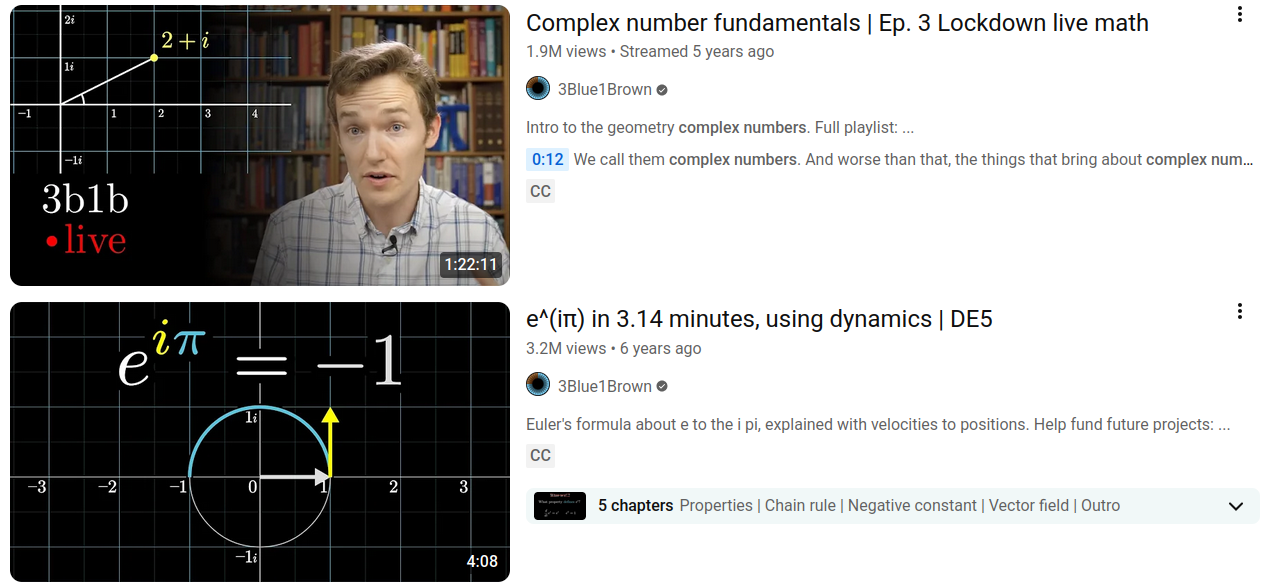
\includegraphics[width=\linewidth]{../figures/3b1b_complexes.png}
  \end{center}
\end{frame}

\begin{frame}{Quaternions and 3D rotations}
  Quaternions extend complex numbers for 3D rotations.
  
  \bigskip
  Numbers $1, i, j, k$ with the multiplication table:
  
  \begin{center}
  \begin{tabular}{c|cccc}
    $\times$ & $1$ & $i$ & $j$ & $k$ \\
    \hline
    $1$ & $1$ & $i$ & $j$ & $k$ \\
    $i$ & $i$ & $-1$ & $k$ & $-j$ \\
    $j$ & $j$ & $-k$ & $-1$ & $i$ \\
    $k$ & $k$ & $j$ & $-i$ & $-1$
  \end{tabular}
  \end{center}
  
  \bigskip
  Used in 3D graphics and video games. In physics, Pauli matrices are preferred.

  \bigskip
  This exercise can be continued with more general transformations than rotations: this leads to \textbf{group theory} and their representations.
  
\end{frame}

\begin{frame}{Summary $\mathbb{C}$}

  \vspace{2mm}
  \begin{itemize}
    \setlength{\itemsep}{0.9em}
    \item Complex numbers solve the problem of $\sqrt{-1}$
    \item Extension of real numbers by adding a phase $e^{i\theta}$
    \item Three representations: Cartesian, vector, polar
  \end{itemize}

  \begin{center}
    \vspace{2mm}
  \begin{tikzpicture}[scale=1.0]
    \draw[->] (-2.5,0) -- (2.5,0) node[right] {Re};
    \draw[->] (0,-0.5) -- (0,2.5) node[above] {Im};
    \draw[->,thick,blue] (0,0) -- (1,2) node[above right] {$z$};
    \draw[->] (0.8,0.0) arc (0:60:0.8);
    \node at (1.0,0.6) {$e^{i\theta}$};
  \end{tikzpicture}
  \end{center}

\end{frame}

\end{document}
